\section{Plus grand commun diviseur}
\subsection{Définition et propriétés}

\begin{definition}
Soit $a$ et $b$ deux entiers relatifs non tous nuls.

L'ensemble des diviseurs communs à $a$ et $b$ admet un plus grand
élément $d$, appelé plus grand commun diviseur. On le note
: PGDC$(a,b)$.
\end{definition}

\begin{preuve}
\emph{Existence}

L'ensemble des diviseurs communs à $a$ et $b$ est un ensemble fini car c'est l'intersection de deux ensembles finis.

De plus, 1 divise $a$ et $b$ donc l'ensemble des diviseurs communs à $a$ et $b$ est non vide.

Or tout ensemble fini non vide dans $\Z$ admet un plus grand et unique élément, donc $d$ existe.
\end{preuve}

\begin{exemples*1}
$\pgcd(24,18)=6,\enskip \pgcd(60,84)=12,\enskip\pgcd(150,240)=30$.
\end{exemples*1}

\begin{propriete}
\begin{itemize}
\item $\pgcd(a,b)=\pgcd(b,a)$
\item $\pgcd(a,b)=\pgcd(|a|,|b|)$
\item $\pgcd(a,0)=a$\enskip car 0 est multiple de tout entier.
\item Si $b$ divise $a$, alors\enskip $\pgcd(a,b)=|b|$.
\item Pour tout entier naturel $k$ non nul, on a :\enskip $\pgcd(ka,kb)=k\,\pgcd(a,b)$.
\end{itemize}

\vspace{-\baselineskip}
\end{propriete}

\begin{remarque}
Les preuves de ces propriétés sont laissées à l'initiative de l'élève.
\end{remarque}

\begin{exemples*1}
\begin{itemize}
\item $\pgcd(82,0)=82$.
\item $\pgcd(-24,-18)=\pgcd(24,18)=6$.
\item $\pgcd(30,5)=5$\enskip car 30 est un multiple de 5.
\item $\pgcd(240,180)=10\pgcd(24,18)=60$.
\end{itemize}

\vspace{-\baselineskip}
\end{exemples*1}

\subsection{Nombres premiers entre eux}
\begin{definition}
On dit que $a$ et $b$ sont premiers entre eux si $\pgcd(a,b)=1$.
\end{definition}\medskip

\begin{exemple*1}
\begin{itemize} 
\item $\pgcd(15,8)=1$\enskip donc 15 et 8 sont premiers entre eux.
\item $\pgcd(a,1)=1$.\enskip Le nombre 1 est premier avec tout entier.
\end{itemize}
\vspace{-\baselineskip}
\end{exemple*1}

\begin{attention}
  Il ne faut pas confondre des nombres premiers entre eux et des
  nombres\linebreak premiers. 15 et 8 ne sont pas premiers et pourtant ils sont
  premiers entre eux.

Par contre, deux nombres premiers distincts sont nécessairement premiers entre eux.
\end{attention}

\subsection{Algorithme d'Euclide}

\begin{theoreme}
  Soit $a$ et $b$ deux entiers naturels non nuls tels que $b$ ne
  divise pas $a$.

  La suite des divisions euclidiennes suivantes finit par
  s'arrêter. Le dernier reste non nul est alors le PGCD de $a$ et de
  $b$.\vspace{-5pt}
$$\begin{aligned}
\text{Division de $a$ par $b$}\qquad &a=b\,q_0+r_0 \quad&\text{avec}&\quad b>r_0\Sup0\\
\text{Division de $b$ par $r_0$}\qquad &b=r_0\,q_1+r_1 \quad&\text{avec}&\quad r_0>r_1\Sup0\\
\text{Division de $r_0$ par $r_1$}\qquad &r_0=r_1\,q_2+r_2 \quad&\text{avec}&\quad r_1>r_2\Sup0\\
\vdots \hspace{2cm}\null & \qquad\qquad\vdots\\
\text{Division de $r_{n-2}$ par $r_{n-1}$}\qquad &r_{n-2}=r_{n-1}\,q_n+r_n \quad&\text{avec}&\quad r_{n-1}>r_n\Sup0\\
\text{Division de $r_{n-1}$ par $r_n$}\qquad &r_{n-1}=r_n\,q_{n+1}+0 & \\
\end{aligned}$$
On a alors \enskip$\pgcd(a,b)=r_n$.

\end{theoreme}

\begin{preuve}
\begin{itemize}
\item Montrons que\enskip $\pgcd(a,b)=\pgcd(b,r_0)$.\medskip

Soit\enskip $D=\pgcd(a,b)$\enskip et\enskip $d=\pgcd(b,r_0)$.\medskip

$D$ divise $a$ et $b$ donc $D$ divise\enskip $a-bq_0=r_0$,\enskip donc $D$ divise $b$ et $r_0$. Par conséquent $D\Inf d$.

$d$ divise $b$ et $r_0$ donc $d$ divise\enskip $bq_0+r_0=a$,\enskip donc $d$ divise $a$ et $b$. Par conséquent $d\Inf D$.\medskip

On  déduit de ces deux inégalités que\enskip $D=d$, d'où $\pgcd(a,b)=\pgcd(b,r_0)$.\medskip

\item La suite des restes : $r_0$, $r_1$, $r_2$, \dots, $r_n$ est une suite strictement décroissante dans $\N$ car :

$r_0>r_1>r_2> \dots >r_n$. 

D'après le principe de descente infinie, il existe alors $n$ tel que $r_{n+1}=0$.\medskip

\item De proche en proche, on en déduit que : \vspace{-5pt}

$$\pgcd(a,b)=\pgcd(b,r_0)=\dots=\pgcd(r_{n-2},r_{n-1})=\pgcd(r_{n-1},r_n).$$ 

Or $r_n$ divise $r_{n-1}$, donc\enskip $\pgcd(r_{n-1},r_n)=r_n$.\medskip

\item Conclusion :\enskip $\pgcd(a,b)=r_n$.\enskip Le dernier reste non nul est le $\pgcd$.
\end{itemize}
\end{preuve}

\begin{methode*1}[Calculer le PGCD de deux nombres\MethodeRefExercice*{exo-alg_euclide}]
\exercice
\label{methode-alg_euclide}
Calculer $\pgcd(\nombre{4539},\nombre{1958})$.
\correction
On effectue les divisions euclidiennes suivantes :\vspace{-5pt}
$$\begin{aligned}
\nombre{4539}&=\nombre{1958}\times2+623\\
\nombre{1958}&=623\times3+89\\
623&=89\times7
\end{aligned}\vspace{-5pt}$$

Conclusion : $\pgcd(\nombre{4539},\nombre{1958})=89$.
\end{methode*1}

\begin{remarque}
Le petit nombre d'étapes de cet exemple montre la performance de cet algorithme à comparer avec la décomposition en facteurs premiers (voir chapitre A3).

\algo Voir TP 1 pour la performance de l'algorithme.
\end{remarque}


\section{Théorème de Bézout}

\vspace{-5pt}
\parbox{0.7\textwidth}{%
  \begin{minipage}{0.6\textwidth} Sur la pierre tombale d’Étienne
    Bézout (né à Nemours, le 31 mars 1730 et mort aux Basses-Loges, le
    27 septembre 1783), dans l’église Saint-Pierre à
    Avon (en Seine-et-Marne), on peut lire cette épitaphe :

\begin{center}
\ofg{Géomètre savant, philosophe paisible.

Père, époux, citoyen, ami tendre et sensible.

Son savoir fut profond, son esprit pénétrant.

Il connut les plaisirs que donne la sagesse ;

il vécut pour les siens, cultiva leur tendresse

et fit de leur bonheur, son bonheur le plus grand.

Pour sauver de l'oubli son nom et sa mémoire

ce marbre était sans doute un témoin superflu ;

mais des regrets que laisse après lui sa vertu

l'amitié se console en parlant de sa gloire.}
\end{center}

\end{minipage}}
\parbox{0.2\textwidth}{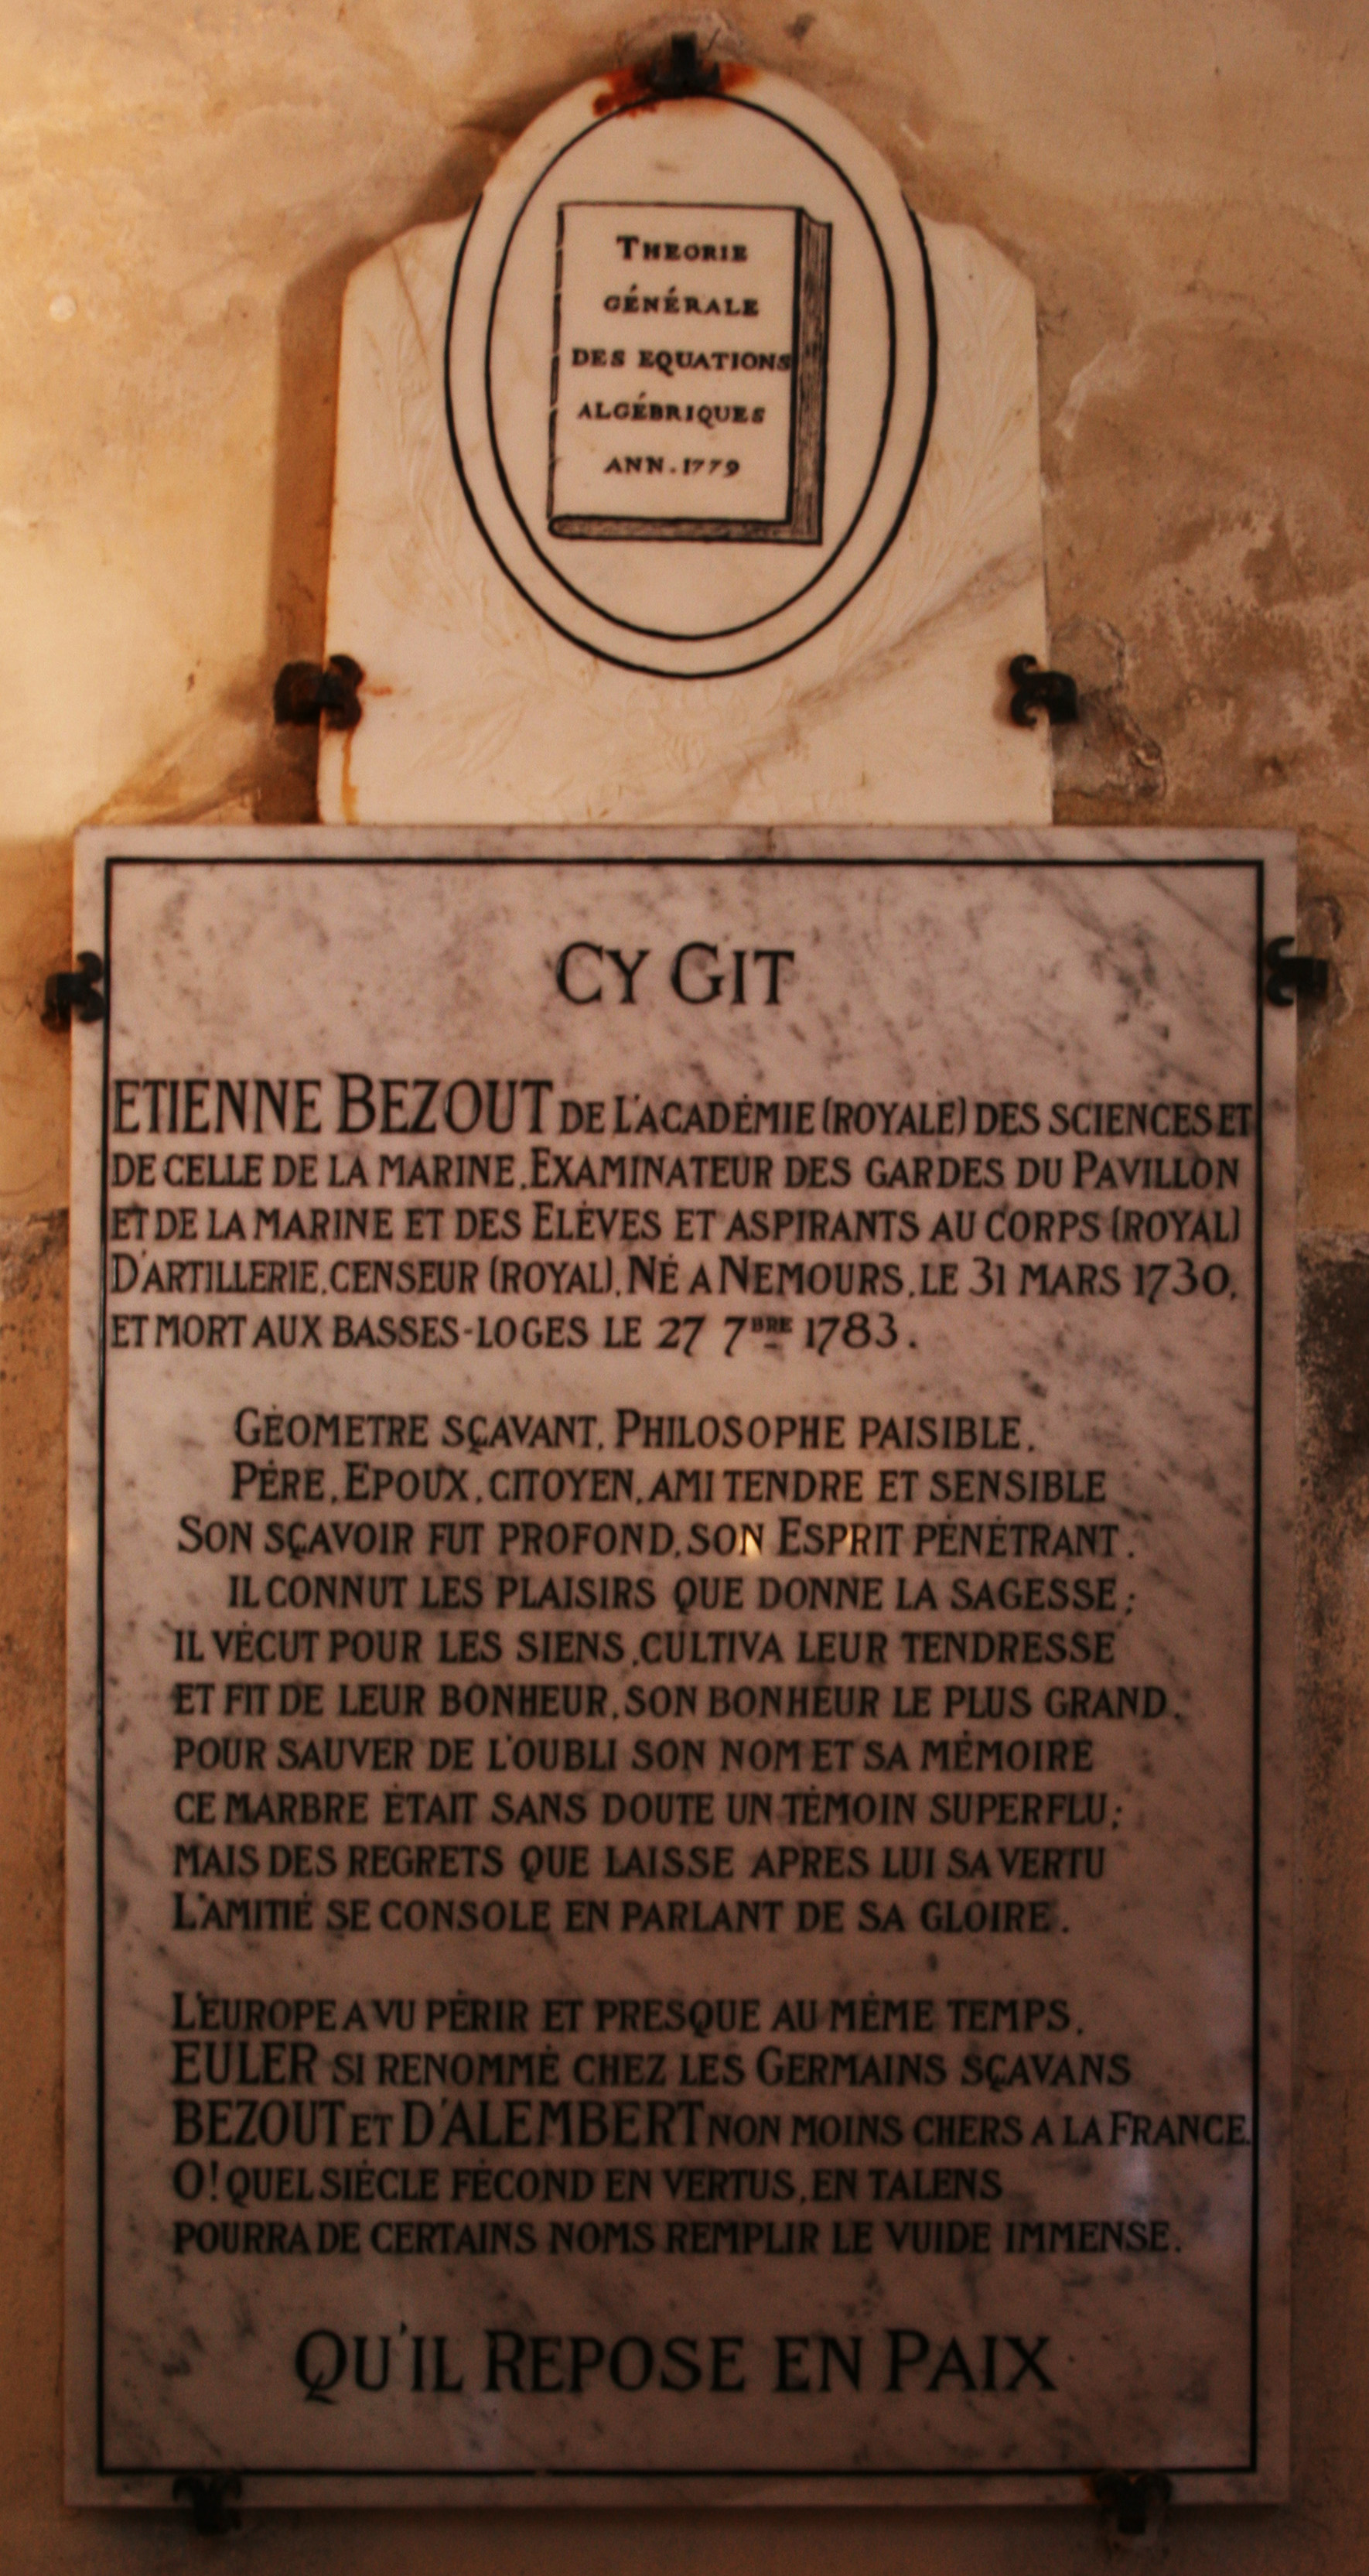
\includegraphics[width=0.20\textwidth]{02_Etienne_Bezout_plaque}}

\subsection{\MotDefinition{Identité de Bézout}[Identité de Bézout]{}}
\begin{propriete}

Soit $a$ et $b$ deux entiers non nuls et $D=\pgcd(a,b)$.

Il existe alors un couple $(u,v)$ d'entiers relatifs telle que :\enskip $au+bv=D$.
\end{propriete}

\begin{preuve}

Soit $G$ l'ensemble formé par les entiers naturels strictement positifs de la forme $ma+nb$ où $m$ et $n$ sont des entiers relatifs.

$G$ est une partie de $\N$ non vide : on vérifie facilement que $\left|a\right|\in G$.\medskip

D'après le principe du bon ordre, $G$ admet donc un plus petit élément
$d$ tel que $d=au+bv$.
\begin{itemize}
\item $D=\pgcd(a,b)$ divise $a$ et $b$ donc $D$ divise\enskip
  $au+bv=d$\enskip et donc\enskip $D\Inf d$.\medskip

\item Montrons que $d$ divise $a$.

Divisons $a$ par $d$, on a alors $a=dq+r$\enskip avec\enskip $0\Inf r<d$.

On  isole le reste et on remplace $d$ par $au+bv$ :\vspace{-10pt}
$$r=a-dq=a-auq-bvq=a(1-uq)+b(-vq)\vspace{-10pt}$$

Si $r\neq0$ alors $r\in G$, or $r<d$ et $d$ est le plus petit élément de $G$, cela est contradictoire.

Donc $r=0$ par conséquent $d$ divise $a$.


\item En faisant le même raisonnement, on montre que $d$ divise aussi $b$.\medskip

$d$ divise $a$ et $b$, donc $d\Inf D$.

\item Conclusion :\enskip $D\Inf d$\enskip et\enskip $d\Inf D$\enskip donc\enskip $D=d$.
\end{itemize}
\end{preuve}

\begin{consequence} Tout diviseur commun à $a$ et $b$ divise leur
  $\pgcd$.
\end{consequence}

\subsection{\MotDefinition{Théorème de Bézout}[Théorème de Bézout]{}}

\begin{theoreme}
  Deux entiers relatifs $a$ et $b$ sont premiers entre eux si, et
  seulement si, il existe deux entiers relatifs $u$ et $v$ tels que :
$$au+bv=1$$
\end{theoreme}

\begin{consequence}
  Si\enskip $\pgcd(a\ ;\ b)=D$,\enskip alors \enskip $a=Da'$\enskip et
  \enskip $b=Db'$\enskip avec \enskip $\pgcd(a'\ ;\ b')=1$
\end{consequence}

\begin{remarque}
  La preuve du théorème de Bézout et de sa conséquence fait l'objet de
  l'exercice~21~p.~39.
\end{remarque}


\begin{methode*1}[Montrer que deux nombres sont premiers entre eux\MethodeRefExercice*{exo-bezout}]
\exercice\label{methode-bezout}

Montrer que $(2n+1)$ et $(3n+2)$ sont premiers entre eux, $n\in\N$.
\correction Il faut prouver qu'il existe des coefficients $u$ et $v$
tels que $u(2n+1)+v(3n+2)=1$.
$$-3(2n+1)+2(3n+2)=-6n-3+6n+4=1$$

$\forall n\in\N$,\enskip il existe\enskip $u=-3$ \enskip et\enskip
$v=2$\enskip tels que\enskip $u(2n+1)+v(3n+2)=1$.\medskip

Les entiers $(2n+1)$ et $(3n+2)$ sont donc premiers entre eux.
\end{methode*1}

\begin{methode*1}[Déterminer un couple (\textit{u}\ ;\ \textit{v}) tel que \textit{au}~+~\textit{bv}~=~1\MethodeRefExercice*{exo-sol_particuliere}]
\exercice\label{methode-sol_particuliere}

Montrer que 59 et 27 sont premiers entre eux, puis déterminer un couple d'entiers relatifs $(x,y)$ tel que : \enskip $59x+27y=1$.

\correction

\vspace{-5mm}
\begin{multicols}{2}
Pour montrer que 59 et 27 sont premiers entre eux, on effectue
l'algorithme d'Euclide. 
\begin{center}
$\begin{aligned}
59&=27\times2+5\qquad\hskip-1.7mm (1)\\
27&=5\times5+2\qquad (2)\\
5&=2\times2+1\qquad (3)\end{aligned}$
\end{center}\medskip

Le dernier reste est 1. Donc $\pgcd(59,27)=1$ et 59 et 27 sont premiers entre eux.
\vspace*{4cm}

\columnbreak 

Pour déterminer un couple $(x\ ;\ y)$, on remonte l'algorithme
d'Euclide : 

de (3) on obtient :
\begin{center}$\begin{aligned}
&2\times2=5-1\\
\end{aligned}$\end{center}
On multiplie l'égalité (2) par 2
\begin{center}$\begin{aligned}
&27\times2=5\times10+2\times2\\
&27\times2=5\times10+5-1\\
&27\times2=5\times11-1\\
&5\times11=27\times2+1\\
\end{aligned}$
\end{center}
On multiplie l'égalité (1) par 11
\begin{center}
$\begin{aligned}
\hspace{0.8cm}&59\times11=27\times22+5\times11\\
&59\times11=27\times22+27\times2+1\\
&59\times11=27\times24+1\\
\end{aligned}$
\end{center}
On a donc :
\begin{center}
$\begin{aligned}
\hspace{0.5cm}&59\times11+27\times(-24)=1
\end{aligned}$
\end{center}
\end{multicols}

\vspace{-5mm}
\end{methode*1}

\subsection{\MotDefinition{Corollaire de Bézout}[Corollaire de Bézout]{}}

\begin{propriete}

L'équation\enskip $ax+by=c$\enskip admet des solutions entières si, et seulement si, $c$ est un multiple du $\pgcd(a,b)$.
\end{propriete}

\begin{preuve}
\begin{itemize}
\item \emph{Dans le sens direct} : Supposons que l’équation $ax+by=c$
  admette une solution $(x_0\ ;\ y_0)$.

  Soit $D=\pgcd(a,b)$ alors, comme $D$ divise $a$ et $b$, il divise
  $ax_0+by_0$.

  $D$ divise donc $c$.\medskip

\item \emph{Réciproquement} : Soit $c$ un multiple de $D=\pgcd(a,b)$.

  Donc il existe un entier relatif $k$ tel que : $c=kD$.

  De l'égalité de Bézout, il existe deux entiers relatifs $u$ et $v$
  tels que :\enskip $au+bv=D$.

  En multipliant par $k$, on obtient :\enskip
  $auk+bvk=kD\ \Leftrightarrow\ a(uk)+b(vk)=c$.

  Donc il existe $x_0=uk$ et $y_0=vk$ tels que $ax_0+by_0=c$.
\end{itemize}
\end{preuve}

\begin{exemple*1}
\begin{itemize}
\item L'équation\enskip $4x+9y=2$\enskip admet des solutions car $\pgcd(4,9)=1$\enskip et 2 est multiple de 1.

  En effet, si \enskip $x=-4$\enskip et \enskip $y=2$,\enskip on a :
  \enskip $4(-4)+9(2)=-16+18=2$.

\item L'équation \enskip $9x-15y=2$ \enskip n'admet pas de solution car $\pgcd(9,15)=3$\enskip  et 2 n'est pas multiple de 3.
\end{itemize}
\vspace{-\baselineskip}
\end{exemple*1}

\section{Le théorème de Gauss et son corollaire}

\subsection{\MotDefinition{Théorème de Gauss}[Théorème de Gauss]{}}

\begin{theoreme}
Soit $a$, $b$ et $c$ trois entiers relatifs non nuls.

Si $a$ divise le produit $bc$ et si $a$ et $b$ sont premiers entre eux, alors $a$ divise $c$.
\end{theoreme}

\begin{preuve}
Si $a$ divise le produit $bc$, alors il existe un entier $k$ tel que :\enskip $bc=ka$.\medskip

Si $a$ et $b$ sont premiers entre eux, d'après le théorème de Bézout, il existe deux entiers $u$ et $v$ tels que :\enskip $au+bv=1$.\medskip

En multipliant par $c$, on a :\vspace{-10pt}
$$\begin{aligned}
acu+bcv&=c \qquad \text{or\enskip $bc=ka$,\enskip donc :}\\
acu+kav&=c\\
a(cu+kv)&=c
\end{aligned}\vspace{-5pt}$$

Donc $a$ divise $c$.
\end{preuve}

\begin{exemple*1}
Pour trouver les solutions dans $\Z^2$ de l'équation \enskip $5(x-1)=7y$,\enskip on sait que :\medskip

5 divise $7y$. Or $\pgcd(5,7)=1$,\enskip donc, d'après le théorème de
Gauss, 5 divise $y$.

On a donc : \enskip $y=5k$.\medskip

En remplaçant dans l'équation, on a : \vspace{-10pt}

$$5(x-1)=7\times5k\quad\Leftrightarrow\quad x-1=7k \quad\Leftrightarrow\quad x=7k+1$$

Les solutions sont donc de la forme : \enskip $\left\{\begin{aligned}
x&=7k+1\\
y&=5k\end{aligned}\right.\enskip,\enskip k\in\Z.$\medskip

Réciproquement, ces solutions vérifient effectivement l’équation.
\end{exemple*1}

\subsection{\MotDefinition{Corollaire de Gauss}[Corollaire de Gauss]{}}
\begin{propriete}
Si $b$ et $c$ divisent $a$ et si $b$ et $c$ sont premiers entre eux, alors $bc$ divise $a$.
\end{propriete}

\begin{preuve}
  Si $b$ et $c$ divisent $a$, alors il existe deux entiers relatifs
  $k$ et $k'$ tels que :\vspace{-5pt}
$$a=kb\hspace{0.5cm}\text{et}\hspace{0.5cm} a=k'c\hspace{0.5cm}\text{donc : }\hspace{0.5cm} kb=k'c.\vspace{-5pt}$$

$b$ divise $k'c$, or $\pgcd(b,c)=1$ donc, d'après le théorème de
Gauss, $b$ divise $k'$ donc : \enskip $k'=k''b$.\vspace{-5pt}
$$a=k'c=k''bc\vspace{-5pt}$$

Donc $bc$ divise $a$.
\end{preuve}

\begin{exemple*1}
Si 5 et 12 divisent $a$, comme 5 et 12 sont premiers entre eux,\enskip $5\times12=60$\enskip divise $a$.
\end{exemple*1}

\section{Équation diophantienne \textit{ax} + \textit{by} =
  \textit{c}}

\subsection{Définition et existence}
\begin{definition}
  Une \MotDefinition{équation diophantienne}{} est une équation à
  coefficients entiers dont on cherche les solutions entières. Soit
  $a$, $b$ et $c$ trois entiers relatifs, les équations diophantiennes
  du premier degré sont du type : \enskip $ax+by=c$.
\end{definition}

\begin{remarque}
  Diophante d'Alexandrie est un mathématicien grec du III\ieme{}
  siècle de notre ère.
\end{remarque}

\begin{propriete}
  Une équation diophantienne du premier degré, de la forme $ax+by=c$,
  où $a$, $b$ et $c$ sont des entiers relatifs, admet des solutions
  si, et seulement si, $c$ est un multiple du $\pgcd(a,b)$.
\end{propriete}

\begin{preuve}
  Cela découle directement du corollaire du théorème de Bézout.
\end{preuve}

\begin{exemple*1}
  L'équation \enskip $17x-33y=1$\enskip admet des solutions car
  $\pgcd(17,33)=1$.
\end{exemple*1}

\subsection{Résolution}

\begin{methode*1}[Résoudre une équation du type \textit{ax} + \textit{by} = \textit{c}\MethodeRefExercice*{exo-eq_diophantienne}]
\begin{itemize}
\item On cherche une solution particulière à l'équation.

\item On recherche ensuite l'ensemble des solutions en soustrayant termes à termes l'équation et l'égalité de la solution particulière.

\item On applique le théorème de Gauss, puis l'on vérifie que les solutions trouvées vérifient bien l'équation.
\end{itemize}
\exercice
\label{methode-eq_diophantienne}
Déterminer l'ensemble des solutions de l'équation (E) \enskip $17x-33y=1$.
\correction
\begin{enumerate}
\item On cherche une solution particulière de (E). Ici, il existe une
  solution évidente : le couple (2;1), car \enskip $17\times2-33\times1=34-33=1$.\medskip
\item On recherche ensuite la solution générale de (E).
On a : \enskip $\left\{\begin{aligned}
&17x\enskip -\enskip 33y\enskip=1\\
&17\times 2 - 33 \times 1 = 1\end{aligned}\right.$.

Par soustraction termes à termes des deux égalités, on obtient :
$$17(x-2)-33(y-1)=0\enskip\Leftrightarrow\enskip 17(x-2)=33(y-1)\quad (\text{E'})$$

33 divise $17(x-2)$. Or $\pgcd(17,33)=1$, donc d'après le théorème de
Gauss, 33 divise $(x-2)$. On a donc : \enskip
$x-2=33\,k,\enskip k\in\Z$. En remplaçant dans (E'), on trouve \enskip
$y-1=17\,k$.\medskip

\item Les  solutions de (E) sont de la forme : \enskip $\left\{\begin{aligned}
&x=2+33\,k\\
&y=1+17\,k\end{aligned}\right.\enskip, \enskip k\in\Z.$\medskip

\item Ces solutions vérifient effectivement l’équation.
\end{enumerate}
\exercice
Déterminer l'ensemble des solutions de l'équation (E$_1$) \enskip $15x+8y=5$.
\correction
\begin{enumerate}
\item L'équation (E$_1$) admet des solutions car 15 et 8 sont premiers entre eux.
\item On cherche une solution particulière à l'équation (E$_2$) : \enskip $15x+8y=1$.

$(-1~;~2)$ est solution évidente à (E$_2$) car : \enskip $15\times(-1)+8\times2=-15+16=1$.
\item En multipliant par 5, on trouve alors une solution particulière à (E$_1$). Le couple $(-5~;~10)$ est solution de (E$_1$).
\item On recherche ensuite la solution générale de (E$_1$).
On a : \enskip $\left\{\begin{aligned}
&15x\enskip +\enskip 8y\enskip=5\\
&15(-5)+8(10)=5\end{aligned}\right..$

Par soustraction termes à termes des deux égalités on obtient :
{\centering $15(x+5)+8(y-10)=0\enskip\Leftrightarrow\enskip 15(x+5)=8(10-y)\quad (\text{E}_2)$\par}

8 divise $15(x+5)$. Or $\pgcd(15,8)=1$, donc d'après le théorème de
Gauss, 8 divise $(x+5)$. 

On a donc : \enskip $x+5=8\,k,\enskip k\in\Z$. 

En remplaçant dans l'équation (E$_2$), on trouve \enskip
$10-y=15\,k$.\medskip

\item Les  solutions de (E$_1$) sont de la forme : \enskip $\left\{\begin{aligned}
&x=-5+8\,k\\
&y=10-15\,k\end{aligned}\right.\enskip, \enskip k\in\Z$.\medskip

\item Ces solutions vérifient effectivement l’équation.
\end{enumerate}
\vspace{-\baselineskip}
\end{methode*1}

